\begin{figure}
\centering
\begin{subfigure}{.3225\linewidth}
\centering
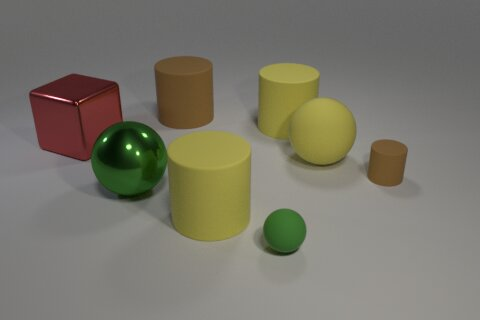
\includegraphics[width=\linewidth]{figures/clevr/input/2.jpg}\\
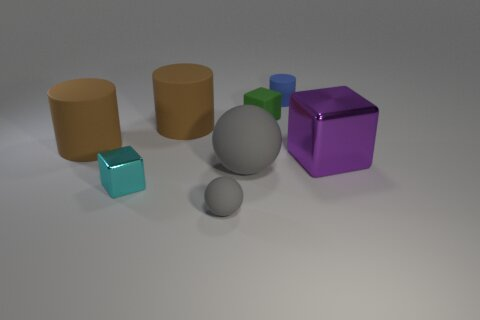
\includegraphics[width=\linewidth]{figures/clevr/input/3.jpg}\\
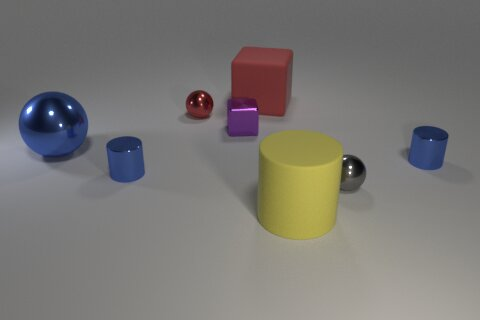
\includegraphics[width=\linewidth]{figures/clevr/input/4.jpg}\\
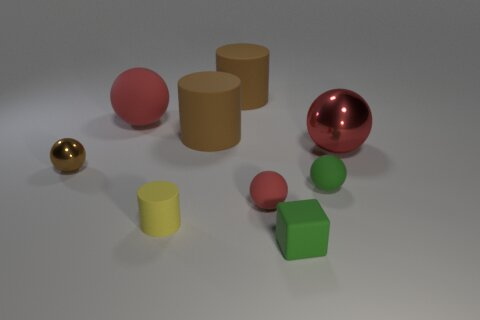
\includegraphics[width=\linewidth]{figures/clevr/input/5.jpg}\\
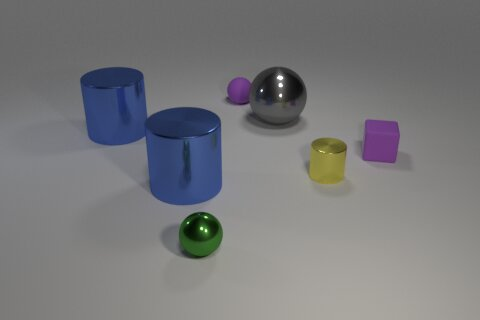
\includegraphics[width=\linewidth]{figures/clevr/input/6.jpg}\\
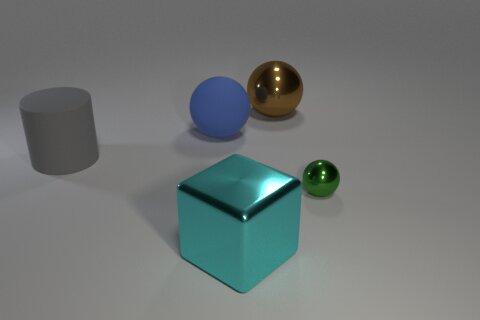
\includegraphics[width=\linewidth]{figures/clevr/input/7.jpg}
\caption{Input}
\end{subfigure}
\hfill
\begin{subfigure}{.3225\linewidth}
\centering
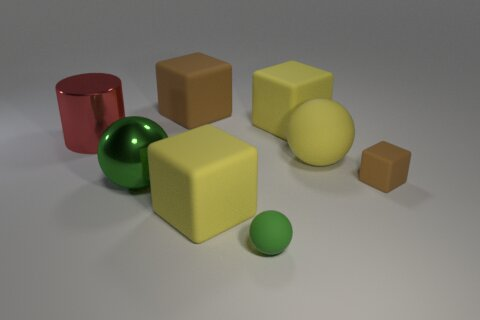
\includegraphics[width=\linewidth]{figures/clevr/ns-vqa/2.jpg}\\
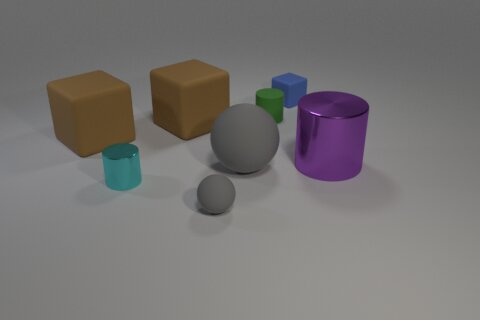
\includegraphics[width=\linewidth]{figures/clevr/ns-vqa/3.jpg}\\
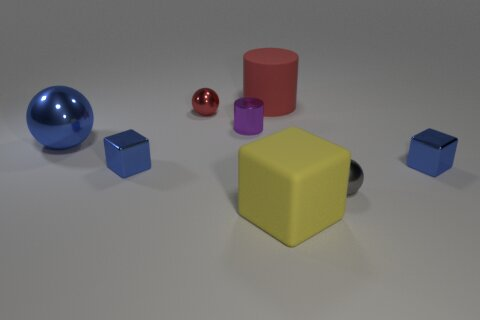
\includegraphics[width=\linewidth]{figures/clevr/ns-vqa/4.jpg}\\
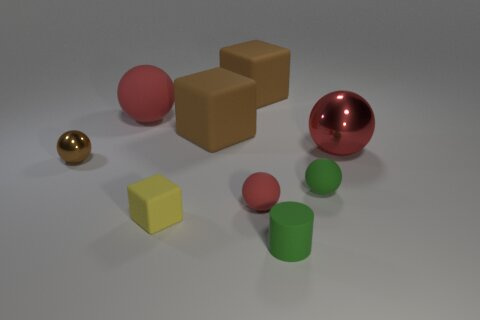
\includegraphics[width=\linewidth]{figures/clevr/ns-vqa/5.jpg}\\
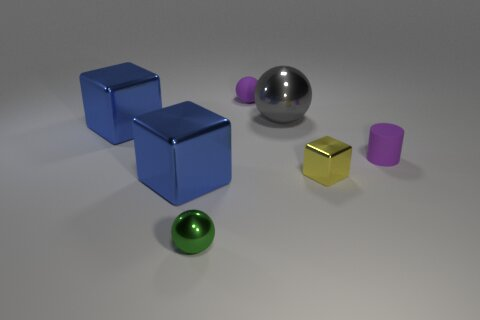
\includegraphics[width=\linewidth]{figures/clevr/ns-vqa/6.jpg}\\
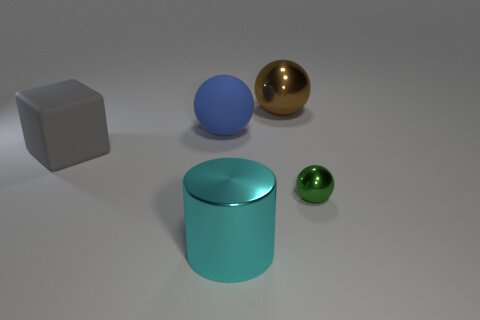
\includegraphics[width=\linewidth]{figures/clevr/ns-vqa/7.jpg}
\caption{NS-VQA}
\end{subfigure}
\hfill
\begin{subfigure}{.3225\linewidth}
\centering
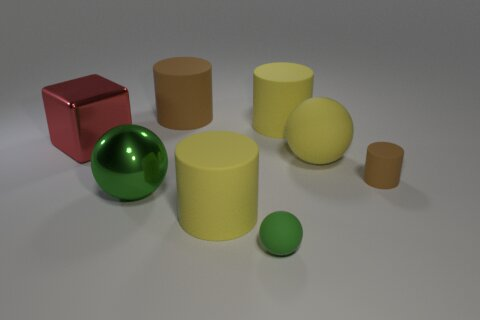
\includegraphics[width=\linewidth]{figures/clevr/output/2.jpg}\\
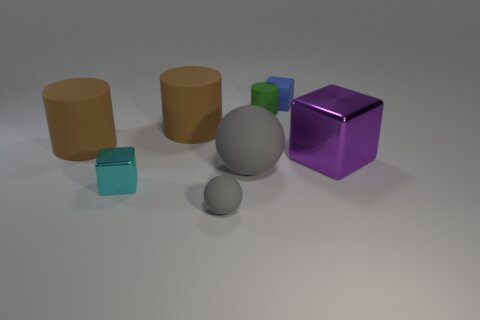
\includegraphics[width=\linewidth]{figures/clevr/output/3.jpg}\\
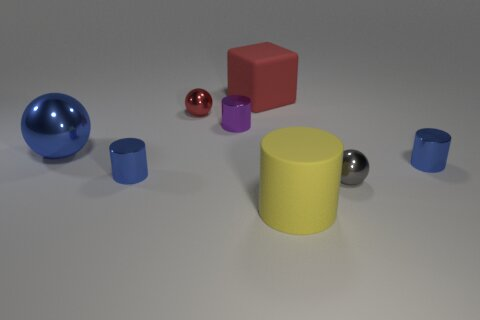
\includegraphics[width=\linewidth]{figures/clevr/output/4.jpg}\\
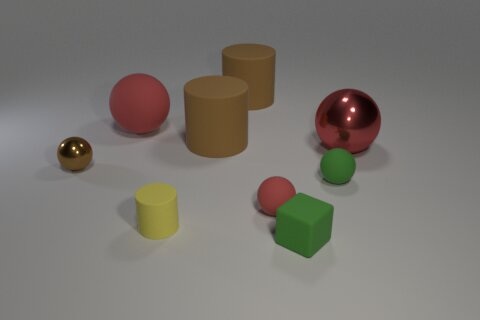
\includegraphics[width=\linewidth]{figures/clevr/output/5.jpg}\\
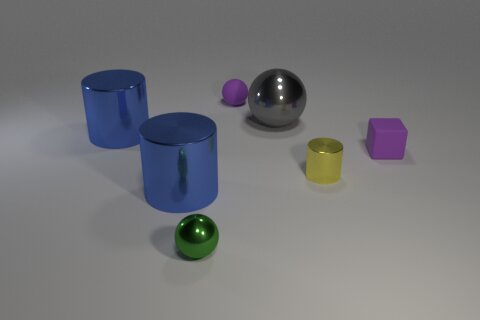
\includegraphics[width=\linewidth]{figures/clevr/output/6.jpg}\\
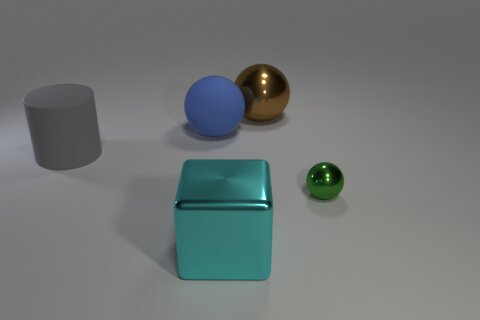
\includegraphics[width=\linewidth]{figures/clevr/output/7.jpg}
\caption{Ours}
\end{subfigure}
\caption{\textbf{Additional OOD CLEVR-CoGenT Samples.} (\cref{ssec:clevr})}
\label{fig:clevr_samples_additional}
\end{figure}
